% Options for packages loaded elsewhere
\PassOptionsToPackage{unicode}{hyperref}
\PassOptionsToPackage{hyphens}{url}
\PassOptionsToPackage{dvipsnames,svgnames,x11names}{xcolor}
%
\documentclass[
  authoryear,
  preprint,
  3p,
  onecolumn]{elsarticle}

\usepackage{amsmath,amssymb}
\usepackage{iftex}
\ifPDFTeX
  \usepackage[T1]{fontenc}
  \usepackage[utf8]{inputenc}
  \usepackage{textcomp} % provide euro and other symbols
\else % if luatex or xetex
  \usepackage{unicode-math}
  \defaultfontfeatures{Scale=MatchLowercase}
  \defaultfontfeatures[\rmfamily]{Ligatures=TeX,Scale=1}
\fi
\usepackage{lmodern}
\ifPDFTeX\else  
    % xetex/luatex font selection
\fi
% Use upquote if available, for straight quotes in verbatim environments
\IfFileExists{upquote.sty}{\usepackage{upquote}}{}
\IfFileExists{microtype.sty}{% use microtype if available
  \usepackage[]{microtype}
  \UseMicrotypeSet[protrusion]{basicmath} % disable protrusion for tt fonts
}{}
\makeatletter
\@ifundefined{KOMAClassName}{% if non-KOMA class
  \IfFileExists{parskip.sty}{%
    \usepackage{parskip}
  }{% else
    \setlength{\parindent}{0pt}
    \setlength{\parskip}{6pt plus 2pt minus 1pt}}
}{% if KOMA class
  \KOMAoptions{parskip=half}}
\makeatother
\usepackage{xcolor}
\setlength{\emergencystretch}{3em} % prevent overfull lines
\setcounter{secnumdepth}{5}
% Make \paragraph and \subparagraph free-standing
\ifx\paragraph\undefined\else
  \let\oldparagraph\paragraph
  \renewcommand{\paragraph}[1]{\oldparagraph{#1}\mbox{}}
\fi
\ifx\subparagraph\undefined\else
  \let\oldsubparagraph\subparagraph
  \renewcommand{\subparagraph}[1]{\oldsubparagraph{#1}\mbox{}}
\fi


\providecommand{\tightlist}{%
  \setlength{\itemsep}{0pt}\setlength{\parskip}{0pt}}\usepackage{longtable,booktabs,array}
\usepackage{calc} % for calculating minipage widths
% Correct order of tables after \paragraph or \subparagraph
\usepackage{etoolbox}
\makeatletter
\patchcmd\longtable{\par}{\if@noskipsec\mbox{}\fi\par}{}{}
\makeatother
% Allow footnotes in longtable head/foot
\IfFileExists{footnotehyper.sty}{\usepackage{footnotehyper}}{\usepackage{footnote}}
\makesavenoteenv{longtable}
\usepackage{graphicx}
\makeatletter
\def\maxwidth{\ifdim\Gin@nat@width>\linewidth\linewidth\else\Gin@nat@width\fi}
\def\maxheight{\ifdim\Gin@nat@height>\textheight\textheight\else\Gin@nat@height\fi}
\makeatother
% Scale images if necessary, so that they will not overflow the page
% margins by default, and it is still possible to overwrite the defaults
% using explicit options in \includegraphics[width, height, ...]{}
\setkeys{Gin}{width=\maxwidth,height=\maxheight,keepaspectratio}
% Set default figure placement to htbp
\makeatletter
\def\fps@figure{htbp}
\makeatother

\usepackage{booktabs}
\usepackage{caption}
\usepackage{longtable}
\usepackage{colortbl}
\usepackage{array}
\usepackage{lineno}\linenumbers \usepackage{multirow} \usepackage{lscape} \newcommand{\blandscape}{\begin{landscape}} \newcommand{\elandscape}{\end{landscape}}
\makeatletter
\@ifpackageloaded{caption}{}{\usepackage{caption}}
\AtBeginDocument{%
\ifdefined\contentsname
  \renewcommand*\contentsname{Table of contents}
\else
  \newcommand\contentsname{Table of contents}
\fi
\ifdefined\listfigurename
  \renewcommand*\listfigurename{List of Figures}
\else
  \newcommand\listfigurename{List of Figures}
\fi
\ifdefined\listtablename
  \renewcommand*\listtablename{List of Tables}
\else
  \newcommand\listtablename{List of Tables}
\fi
\ifdefined\figurename
  \renewcommand*\figurename{Figure}
\else
  \newcommand\figurename{Figure}
\fi
\ifdefined\tablename
  \renewcommand*\tablename{Table}
\else
  \newcommand\tablename{Table}
\fi
}
\@ifpackageloaded{float}{}{\usepackage{float}}
\floatstyle{ruled}
\@ifundefined{c@chapter}{\newfloat{codelisting}{h}{lop}}{\newfloat{codelisting}{h}{lop}[chapter]}
\floatname{codelisting}{Listing}
\newcommand*\listoflistings{\listof{codelisting}{List of Listings}}
\makeatother
\makeatletter
\makeatother
\makeatletter
\@ifpackageloaded{caption}{}{\usepackage{caption}}
\@ifpackageloaded{subcaption}{}{\usepackage{subcaption}}
\makeatother
\journal{Journal Name}
\ifLuaTeX
  \usepackage{selnolig}  % disable illegal ligatures
\fi
\usepackage[]{natbib}
\bibliographystyle{elsarticle-harv}
\usepackage{bookmark}

\IfFileExists{xurl.sty}{\usepackage{xurl}}{} % add URL line breaks if available
\urlstyle{same} % disable monospaced font for URLs
\hypersetup{
  pdftitle={Supplementary Material},
  pdfauthor={Francisco Zambrano; Anton Vrieling; Francisco Meza; Iongel Duran-Llacer; Francisco Fernández; Alejandro Venegas-González; Nicolas Raab; Dylan Craven},
  colorlinks=true,
  linkcolor={blue},
  filecolor={Maroon},
  citecolor={Blue},
  urlcolor={Blue},
  pdfcreator={LaTeX via pandoc}}

\setlength{\parindent}{6pt}
\begin{document}

\begin{frontmatter}
\title{Supplementary Material \\\large{The effects of drought on land
cover change and vegetation productivity in continental Chile} }
\author[1,2]{Francisco Zambrano%
\corref{cor1}%
}
 \ead{francisco.zambrano@umayor.cl} 
\author[3]{Anton Vrieling%
%
}

\author[4,5,6]{Francisco Meza%
%
}

\author[7]{Iongel Duran-Llacer%
%
}

\author[8,9]{Francisco Fernández%
%
}

\author[10]{Alejandro Venegas-González%
%
}

\author[4]{Nicolas Raab%
%
}

\author[12,13]{Dylan Craven%
%
}


\affiliation[1]{organization={Hémera Centro de Observación de la Tierra,
Facultad de Ciencias, Escuela de Ingeniería en Medio Ambiente y
Sustentabilidad, Universidad Mayor},city={Santiago},country={7500994,
Chile.},countrysep={,},postcodesep={}}
\affiliation[2]{organization={Observatorio de Sequía para la Agricultura
y la Biodiversidad de Chile (ODES), Universidad
Mayor},city={Santiago},country={7500994,
Chile.},countrysep={,},postcodesep={}}
\affiliation[3]{organization={Faculty of Geo-Information Science and
Earth, University of Twente},city={Enschede},country={The
Netherlands.},countrysep={,},postcodesep={}}
\affiliation[4]{organization={Facultad de Agronomía y Sistemas
Naturales, Pontificia Universidad Católica de
Chile.},city={Santiago},country={Chile.},countrysep={,},postcodesep={}}
\affiliation[5]{organization={Instituto para el Desarrollo Sustentable.
Pontificia Universidad Católica de
Chile},city={Santiago},country={Chile.},countrysep={,},postcodesep={}}
\affiliation[6]{organization={Centro Interdisciplinario de Cambio
Global, Pontificia Universidad Católica de
Chile},city={Santiago},country={Chile.},countrysep={,},postcodesep={}}
\affiliation[7]{organization={Hémera Centro de Observación de la Tierra,
Facultad de Ciencias, Universidad
Mayor,},city={Santiago},country={7500994,
Chile.},countrysep={,},postcodesep={}}
\affiliation[8]{organization={Center of Economics for Sustainable
Development (CEDES), Faculty of Economics and Government, Universidad
San
Sebastian},city={Santiago},country={Chile.},countrysep={,},postcodesep={}}
\affiliation[9]{organization={Center of Applied Ecology and
Sustainability
(CAPES)},city={Santiago},country={Chile.},countrysep={,},postcodesep={}}
\affiliation[10]{organization={Instituto de Ciencias Agroalimentarias,
Animales y Ambientales (ICA3), Universidad de O'Higgins},city={San
Fernando},country={Chile.},countrysep={,},postcodesep={}}
\affiliation[11]{organization={},,postcodesep={}}
\affiliation[12]{organization={, GEMA Center for Genomics, Ecology \&
Environment, Universidad Mayor, Camino La Pirámide Huechuraba
5750},city={Santiago},country={Chile.},countrysep={,},postcodesep={}}
\affiliation[13]{organization={Data Observatory
Foundation},city={Santiago},country={Chile.},countrysep={,},postcodesep={}}

\cortext[cor1]{Corresponding author}








        





\end{frontmatter}
    
\renewcommand\thesection{S\arabic{section}}
\renewcommand\thefigure{S\arabic{figure}}
\renewcommand\thetable{S\arabic{table}}

\section{Data}\label{data}

\begin{table}

\centering{

[!ht]


\scriptsize
\centering
\begin{tabular}{p{0.1\textwidth}cp{0.3\textwidth}p{0.095\textwidth}ccc}
\hline
\multirow{1}{*}{\centering Product} & Sub-product & Variable & Spatial Resolution  & Period & Units & Short Name \\ 
\hline
\multirow{4}{*}{ERA5L} & ~ & Precipitation & \multirow{4}{*}{~0.1°} & \multirow{4}{*}{1981-2023} & mm & P \\ 
         &  & Maximum temperature & ~ & & $°C$ & $T_{max}$ \\ 
         &  & Minimum temperature & ~ & & $°C$ & $T_{min}$ \\ 
         &  & Volumetric Soil Water Content at 1m & ~ & & $m3/m3$ & SM \\ 
ERA5L* & & Atmospheric Evaporative Demand & 0.1° & 1981-2023 & mm & AED \\
        \multirow{2}{*}{MODIS} & MOD13A3.061 & Normalized Difference Vegetation Index & \multirow{2}{*}{~1 km} & 2000-2023 & ~ & NDVI \\ 
         & MCD12Q1.061 & land cover IGBP scheme & & 2001-2022 & ~ & land cover \\ 
\hline
\end{tabular}
{\raggedright *Calculated from maximum and minimum temperatures derived from ERA5L with Eq. \ref{eq-AED}. \par}

}

\caption{\label{tab-desEOD}Description of the satellite and reanalysis data used}

\end{table}%

\section{Validation of ERA5L
variables}\label{validation-of-era5l-variables}

\subsection{Methods}\label{methods}

We compared the ERA5L \citep{MunozSabater2021} variables for monthly
mean temperature, total precipitation, and volumetric soil water content
against values retrieved by weather stations. For temperature and
precipitation, we used data from the weather network from the Ministry
of Agriculture of Chile (www.agromet.com) between 2015 and 2023. We used
277 stations located throughout Chile. For \emph{in-situ} soil moisture,
we used a private soil network that is owned by the agricultural
enterprise Garces Fruit (https://garcesfruit.com/), which has 99
stations in Central Chile, located in fields with cherry fruit crops.
The sensors are installed at 30, 60, and 90cm and are a Advanced Soil
Moisture Sensor model Teros 12 from the METER Group
(\url{https://metergroup.com/products/teros-12/}). To avoid comparing
ERA5L with \emph{in-situ} soil moisture levels caused by irrigation,
which are not captured by ERA5L, we used daily data for the year 2022
and the months outside the growing season, May to September.

We selected the following metrics:

\[MAE = \frac{1}{n}\sum |{E-S}|\] \[Bias = \frac{\sum E}{\sum S}\]
\[ubRMSE =\sqrt{\frac{\sum{ \left[ (E_i-\overline{E})-(S_i-\overline{S}) \right ] ^2}}{n}}\]

\[CC = \frac{\sum (S_i-\bar{S})(E_i-\bar{E})}{\sqrt{(Si-\bar{S})^2(E_i-\bar{E})^2}}\]

\(MAE\): mean absolute error\\
\(bias\): bias\\
\(ubRMSE\): unbiassed root mean squared error\\
\(CC\): coefficient of correlation\\
\(S\): value of the variable measure by the weather station\\
\(E\): value of the variable measure by ERA5L

\subsection{Results}\label{results}

The average performance metrics of ERA5L over the weather and soil
moisture stations are shown in Table~\ref{tbl-metricsera5}. In the case
of the 97 soil moisture stations, we averaged for the three depths (30,
60, and 90cm) and then compared it with the volumetric water content in
the top 100cm of the soil derived from ERA5L. For this case, we made a
daily comparison to determine the performance metrics per station, then
we averaged the measured soil moisture at the three levels and over all
stations.

\begin{longtable}{lllrr}

\caption{\label{tbl-metricsera5}Metrics of performance for the climatic
and soil moisture variables from ERA5-Land with data from 277 stations
in Central Chile for temperature and precipitation and 99 stations of
soil moisture.}

\tabularnewline

\toprule
Variable & ubRMSE & MAE & Bias & CC \\ 
\midrule\addlinespace[2.5pt]
Temperature & 1.06 °C & 1.13 °C & 1.02 & 0.96 \\ 
Precipitation & 35.5 mm & 28.1 mm & 1.93 & 0.85 \\ 
Soil Moisture (1m) & 0.174 cc/cc & 0.167 cc/cc & 1.74 & 0.71 \\ 
\bottomrule

\end{longtable}

\section{Land cover macroclasses and
validation}\label{land-cover-macroclasses-and-validation}

\subsection{Methods}\label{methods-1}

To analyze the LULCC, we used the IGBP scheme from the MCD12Q1
Collection 6.1 from MODIS. This product has a yearly frequency from 2001
to 2022. The IGBP defines 17 classes; we regrouped these into ten
macroclasses, as follows: classes 1-4 to forest, 5-7 to schrublands, 8-9
to savannas, 10 as grasslands, 11 as wetlands, 12 and 14 to croplands,
13 as urban, 15 as snow and ice, 16 as barren, and 17 to water bodies.

To assess the accuracy of the regrouped MCD12Q1 land cover maps, we
compared the macroclasses with those of a more detailed land cover map
made by \citet{Zhao2016} for Chile with samples acquired in the years
2013--2014 (LCChile). The latter has a spatial resolution of 30 m and
three hierarchy levels of defined classes; from those, we used level 1,
which fits with the macroclass land cover. We chose the years 2013
(IGBP2013) and 2014 (IGBP2014) from the land cover macroclasses to
compare with LCChile. For this comparison, we used the following
procedure:

\begin{enumerate}
\def\labelenumi{\roman{enumi})}
\tightlist
\item
  we resampled LCChile to the spatial resolution (500m) of the land
  cover macroclasses using the majority method,
\item
  we took a random sample of 1000 points within continental Chile and
  extracted the classes that fell within each point for LCChile,
  IGBP2013, and IGBP2014; we considered the point extracted from LCChile
  as the truth and the values from the other two years as predictions.
\item
  we derived a confusion matrix with the classes extracted from the 1000
  points for LCChile, IGBP2013, and IGBP2014; and calculated the
  performance metrics of accuracy and F1.
\end{enumerate}

\[Accuracy = \frac{TP+TN}{TP+TN+FP+FN}=\frac{correct\,\, classifications}{all\,\, classifications}\]
\[F1=\frac{2\cdot TP}{2\cdot TP + FP +FN}\]

where \(TP\) and \(FN\) refer to true positive and false negative,
correctly classified classes; \(TN\) and \(FP\) to true negative and
false positive, wrongly classified classes.

\subsection{Results}\label{results-1}

Our results showed a global accuracy of \textasciitilde0.82 and a F1
score of \textasciitilde0.66 between the high resolution landcover
(LCChile) and the landcover IGBP from MODIS. Thus, for vegetation, we
obtained and use hereafter five macroclasses of land cover from IGBP
MODIS: forest, shrubland, savanna, grassland, and croplands (Table
\ref{tab-landIGBPmacro}).

\begin{table}[!ht]
\caption{Landcover clases from IGBP MODIS and the corresponding macroclasses.}
\label{tab-landIGBPmacro}
\centering
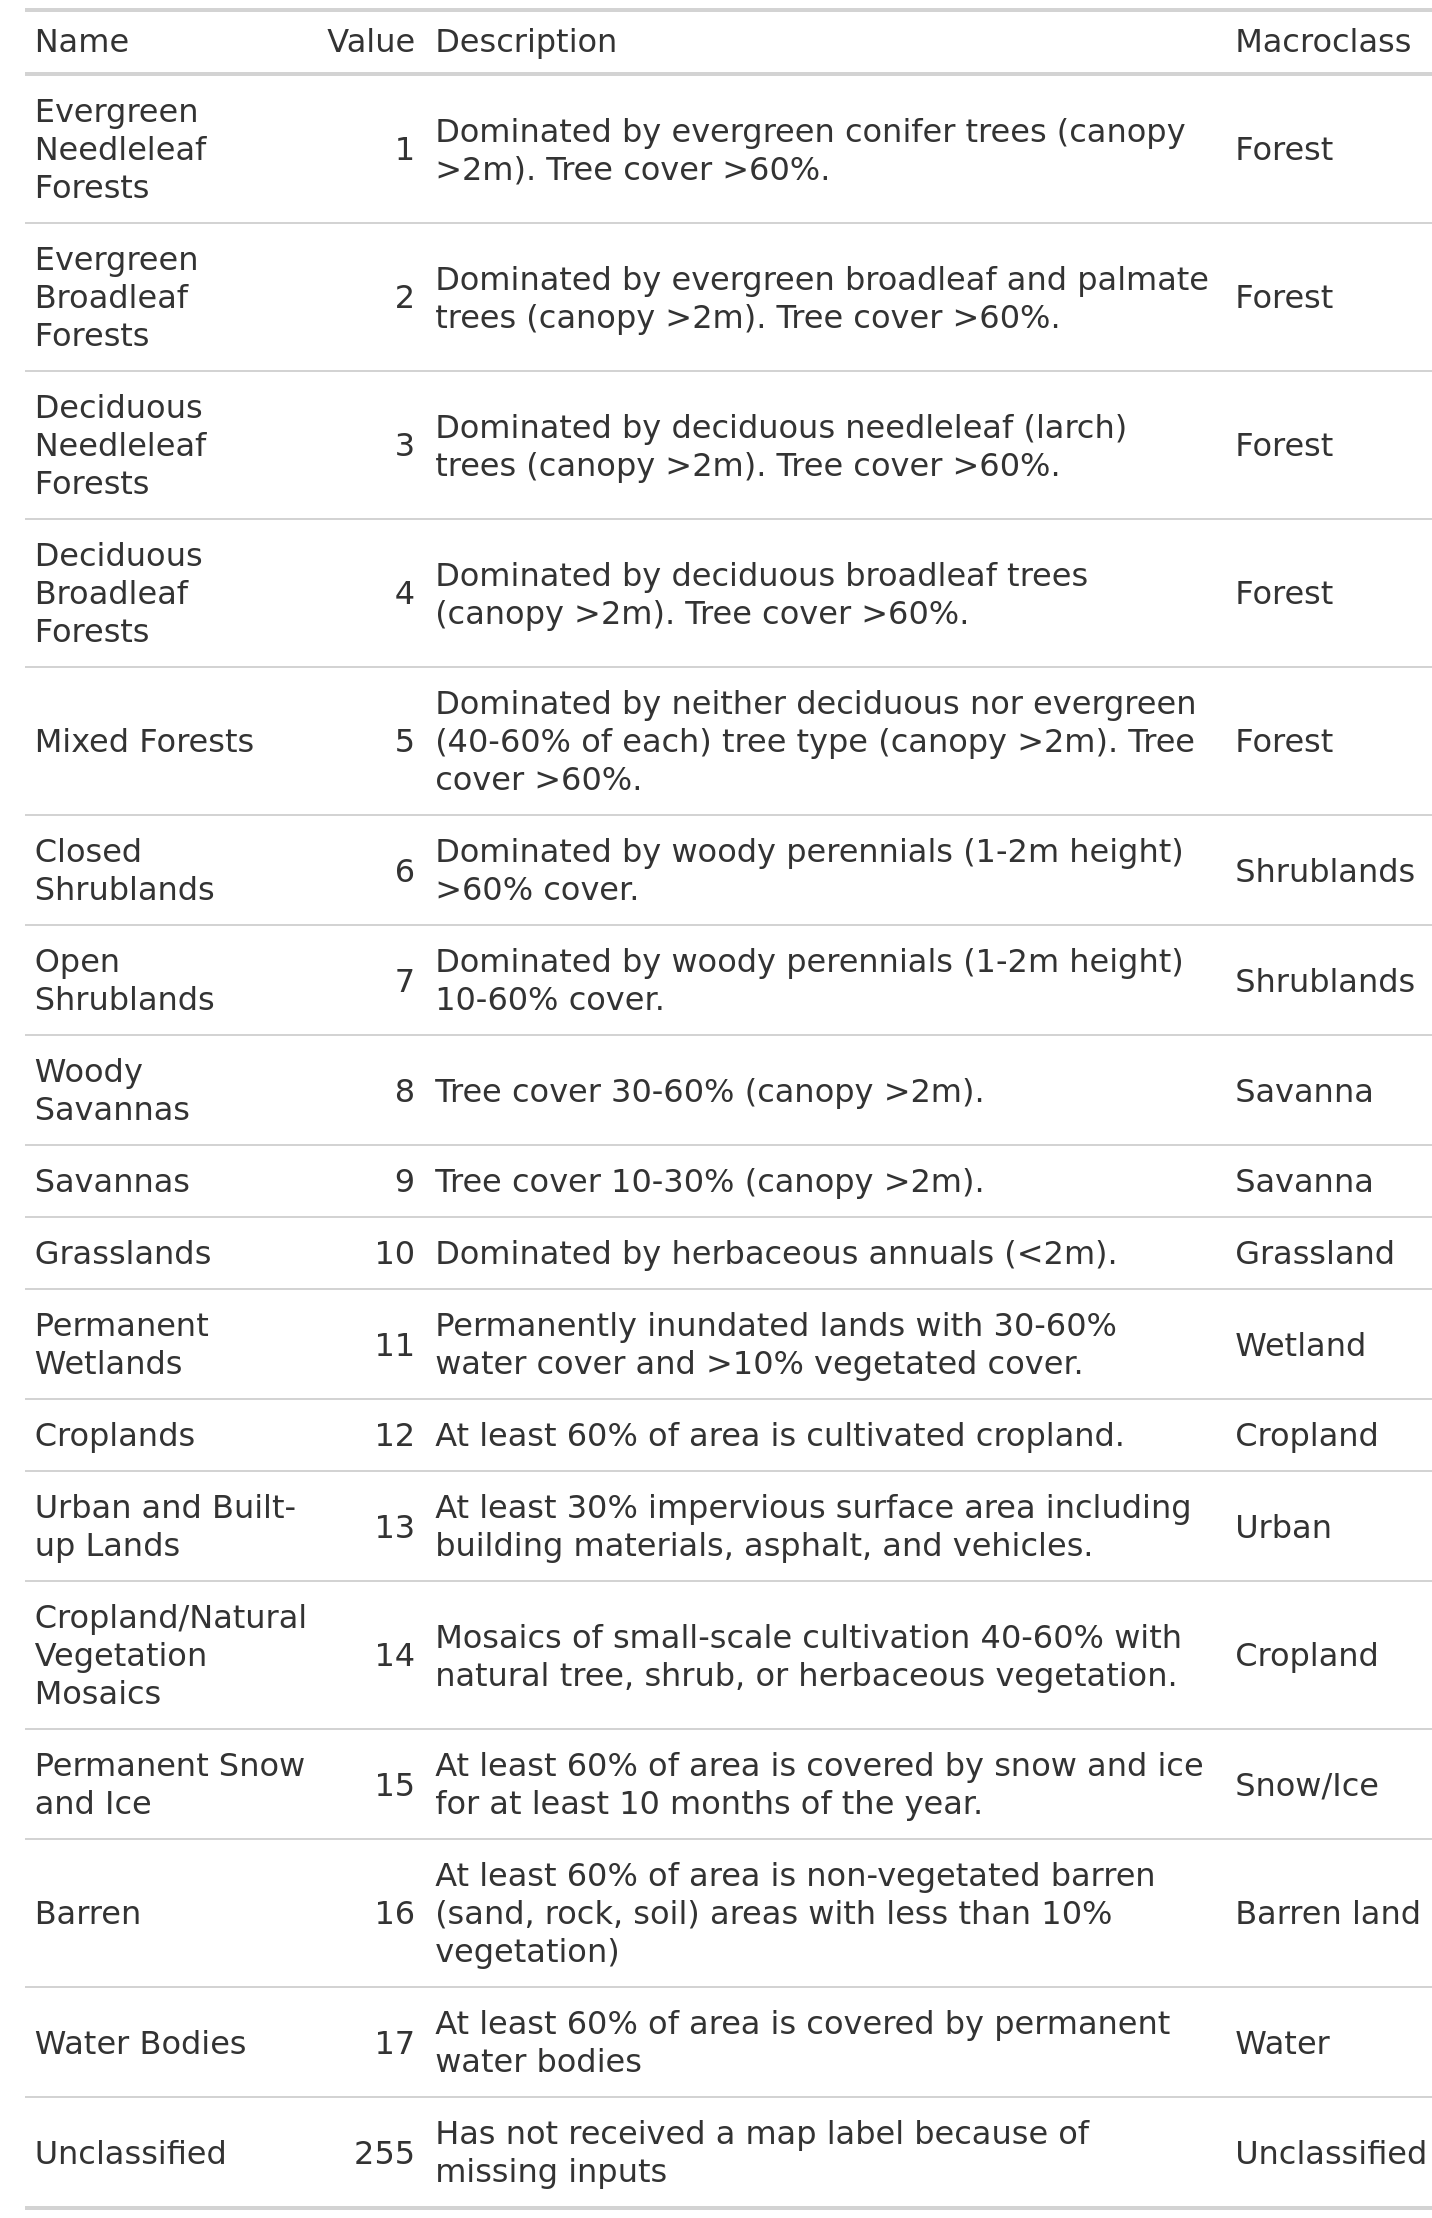
\includegraphics[width = .5\textwidth]{../output/figs/tabla_landcover_macroclass.png}
\end{table}

\section{Relationship between drought indices and land cover
change}\label{relationship-between-drought-indices-and-land-cover-change}

Figure~\ref{fig-RF_importance} shows the ranking of variable importance
obtained with the ten folds used in the resampling of the Random Forest
model per land cover type.

\begin{figure*}[!ht]

\begin{minipage}{0.33\linewidth}

\centering{

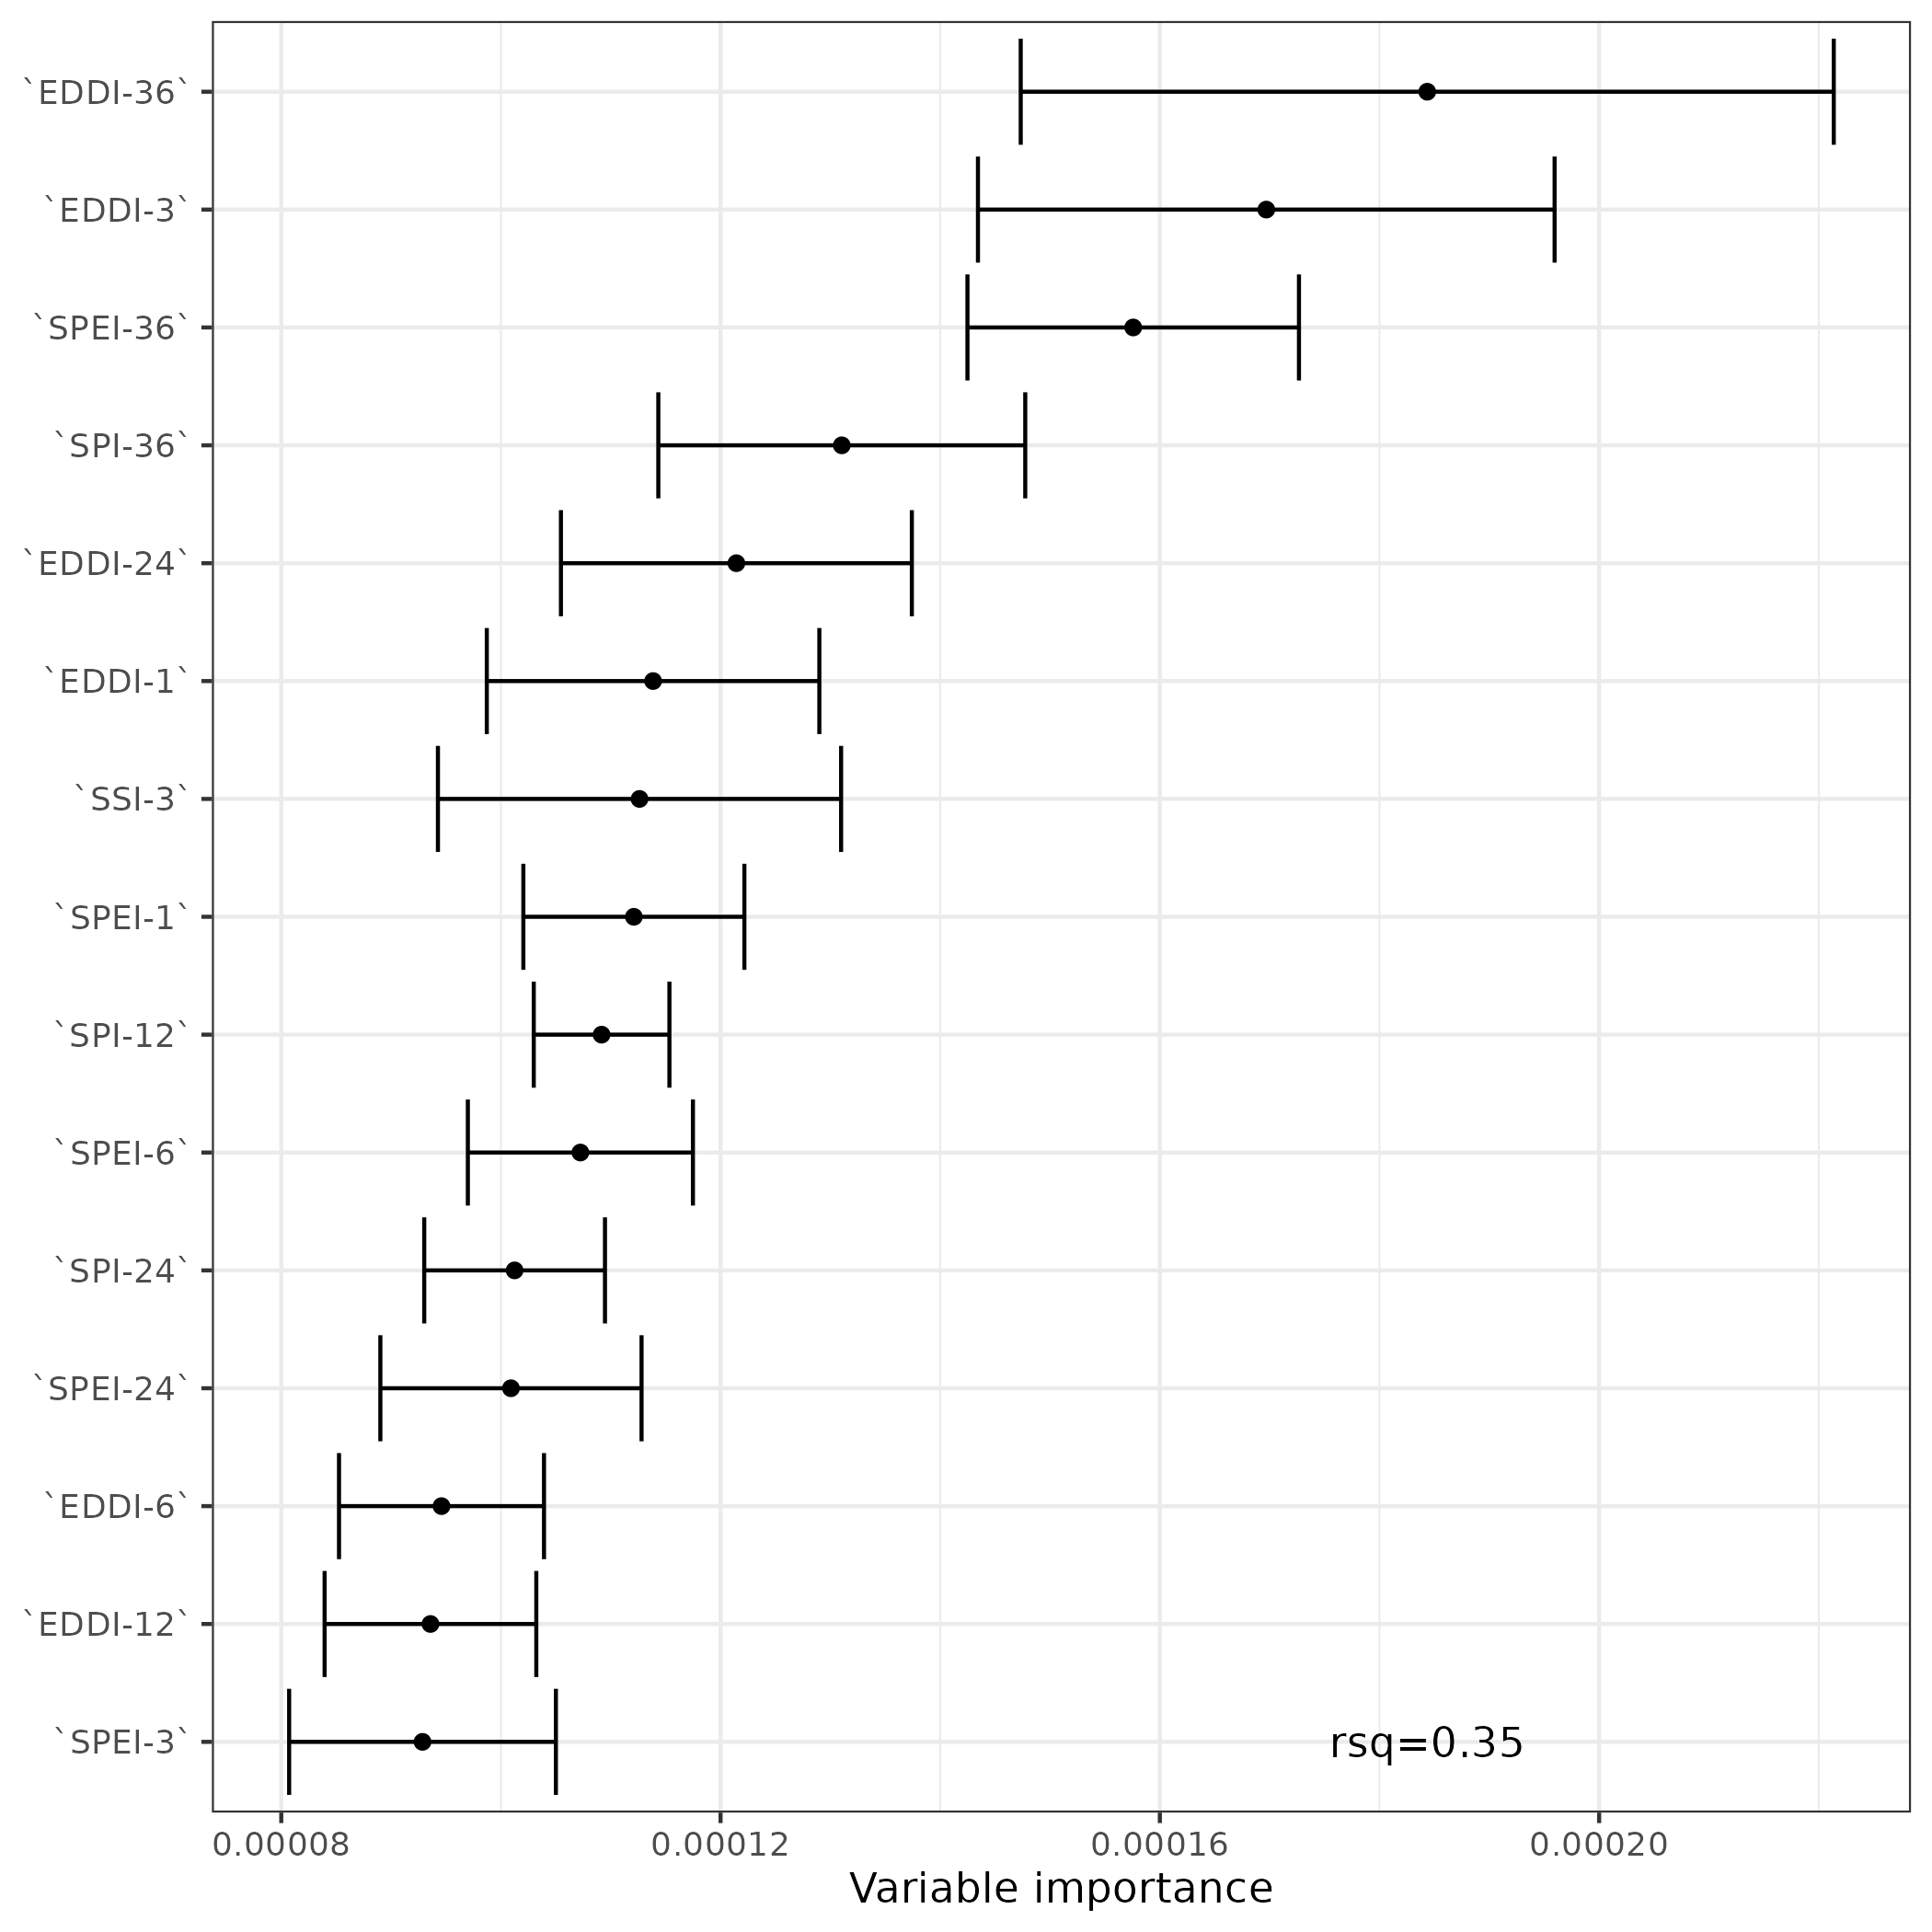
\includegraphics[width=1\textwidth,height=\textheight]{../output/figs/fig_errorbar_resample_random_forest_trends_Forest.png}

}

\subcaption{\label{fig-RF_importance-1}Forest}

\end{minipage}%
%
\begin{minipage}{0.33\linewidth}

\centering{

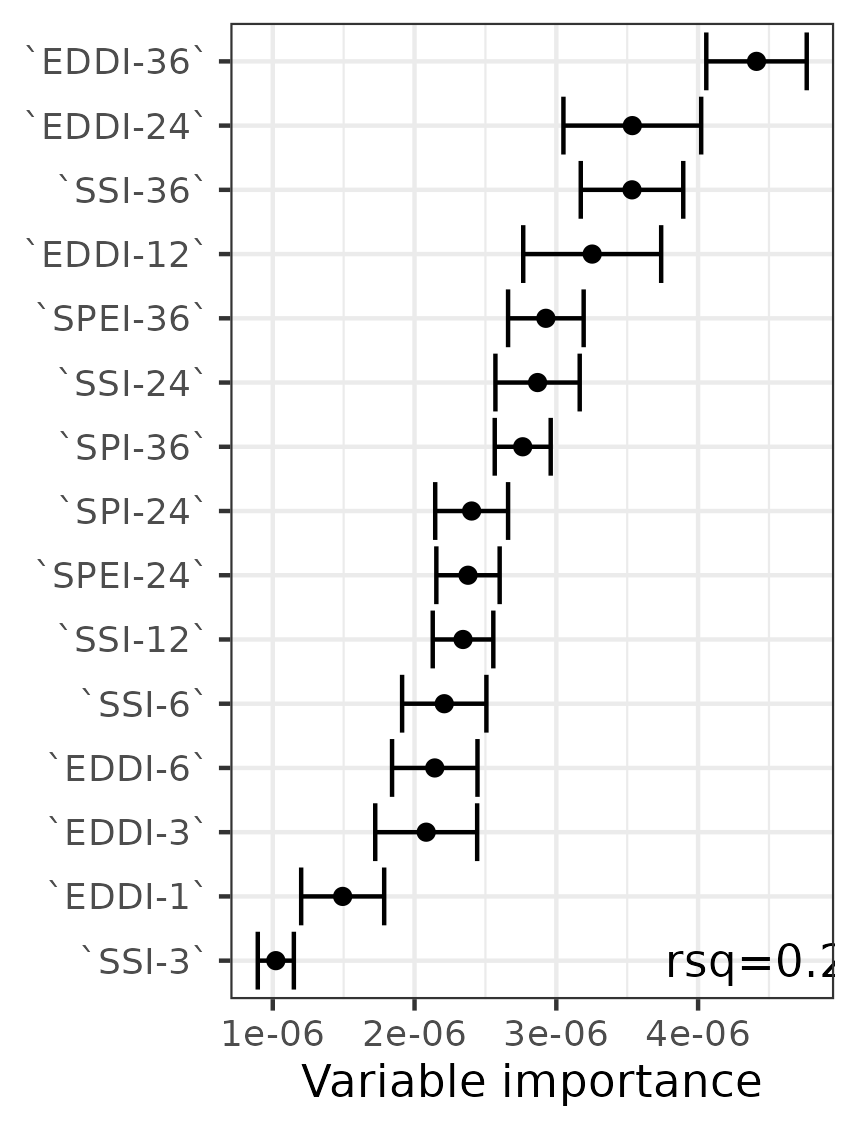
\includegraphics[width=1\textwidth,height=\textheight]{../output/figs/fig_errorbar_resample_random_forest_trends_Cropland.png}

}

\subcaption{\label{fig-RF_importance-2}Cropland}

\end{minipage}%
%
\begin{minipage}{0.33\linewidth}

\centering{

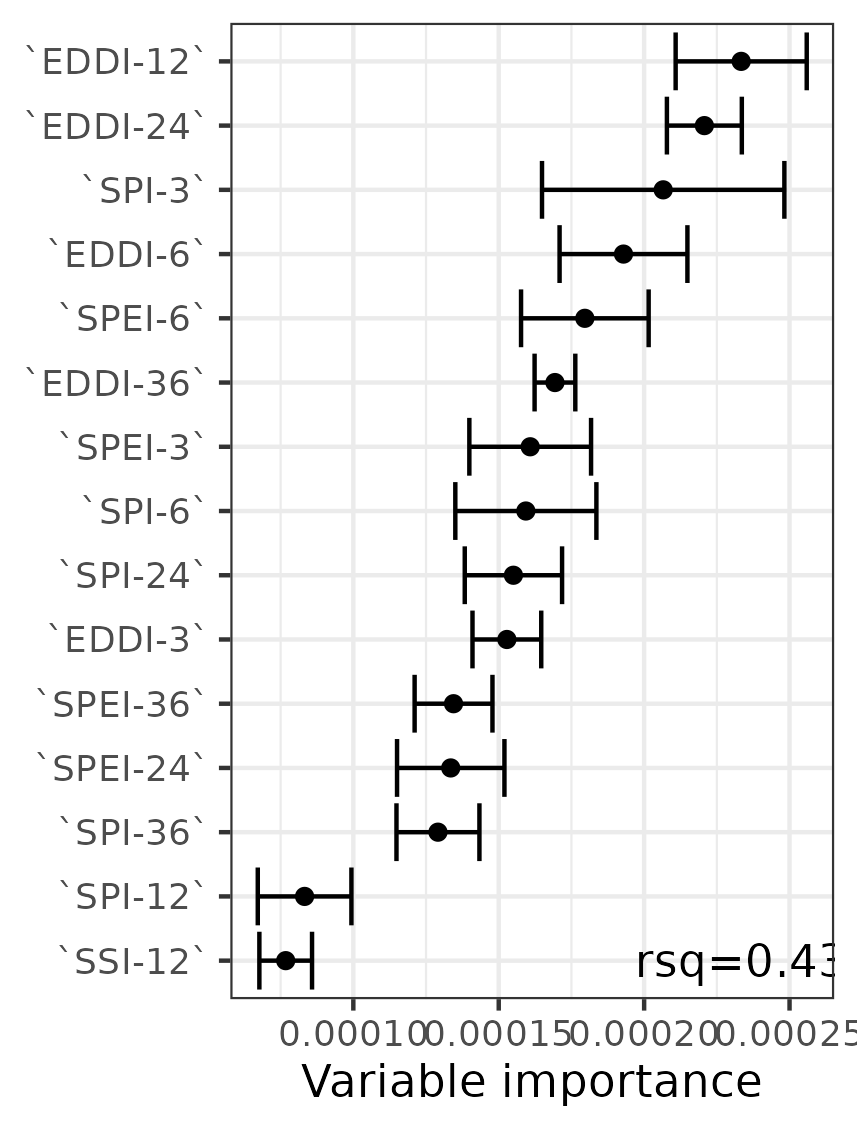
\includegraphics[width=1\textwidth,height=\textheight]{../output/figs/fig_errorbar_resample_random_forest_trends_Grassland.png}

}

\subcaption{\label{fig-RF_importance-3}Grassland}

\end{minipage}%
\newline
\begin{minipage}{0.33\linewidth}

\centering{

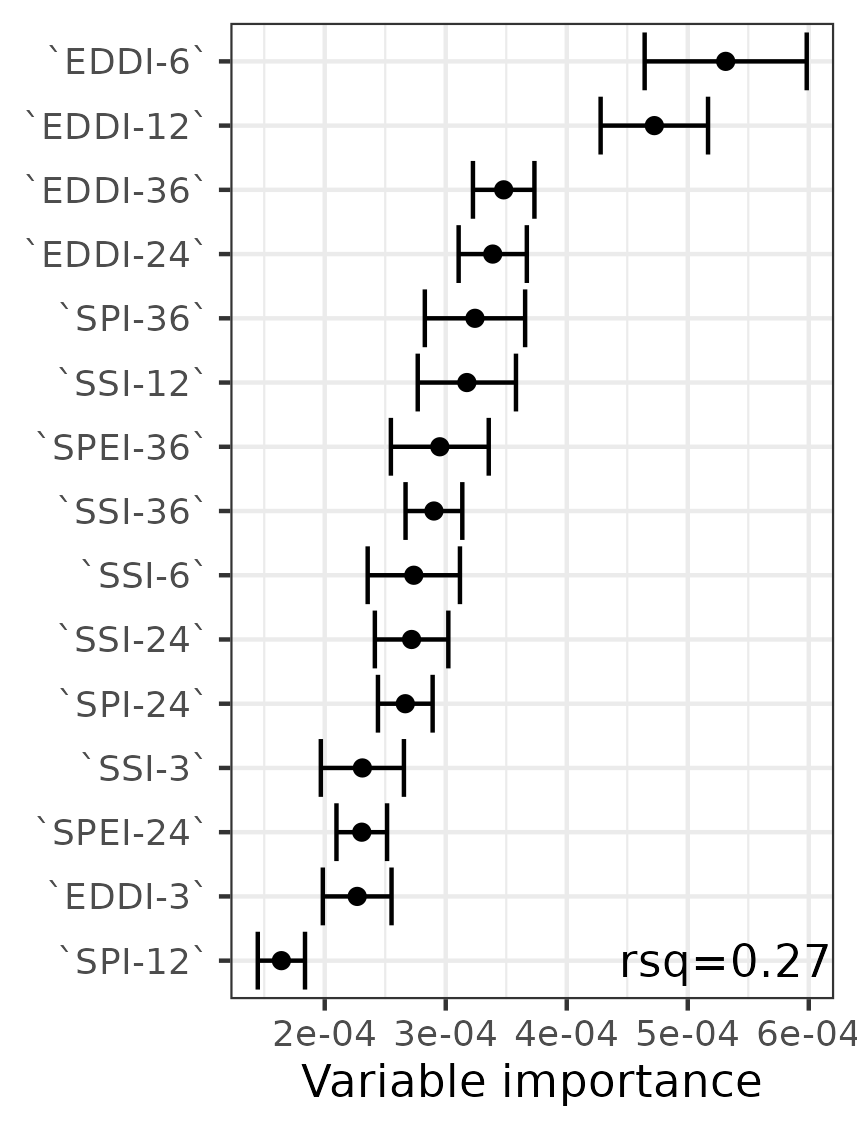
\includegraphics[width=1\textwidth,height=\textheight]{../output/figs/fig_errorbar_resample_random_forest_trends_Savanna.png}

}

\subcaption{\label{fig-RF_importance-4}Savanna}

\end{minipage}%
%
\begin{minipage}{0.33\linewidth}

\centering{

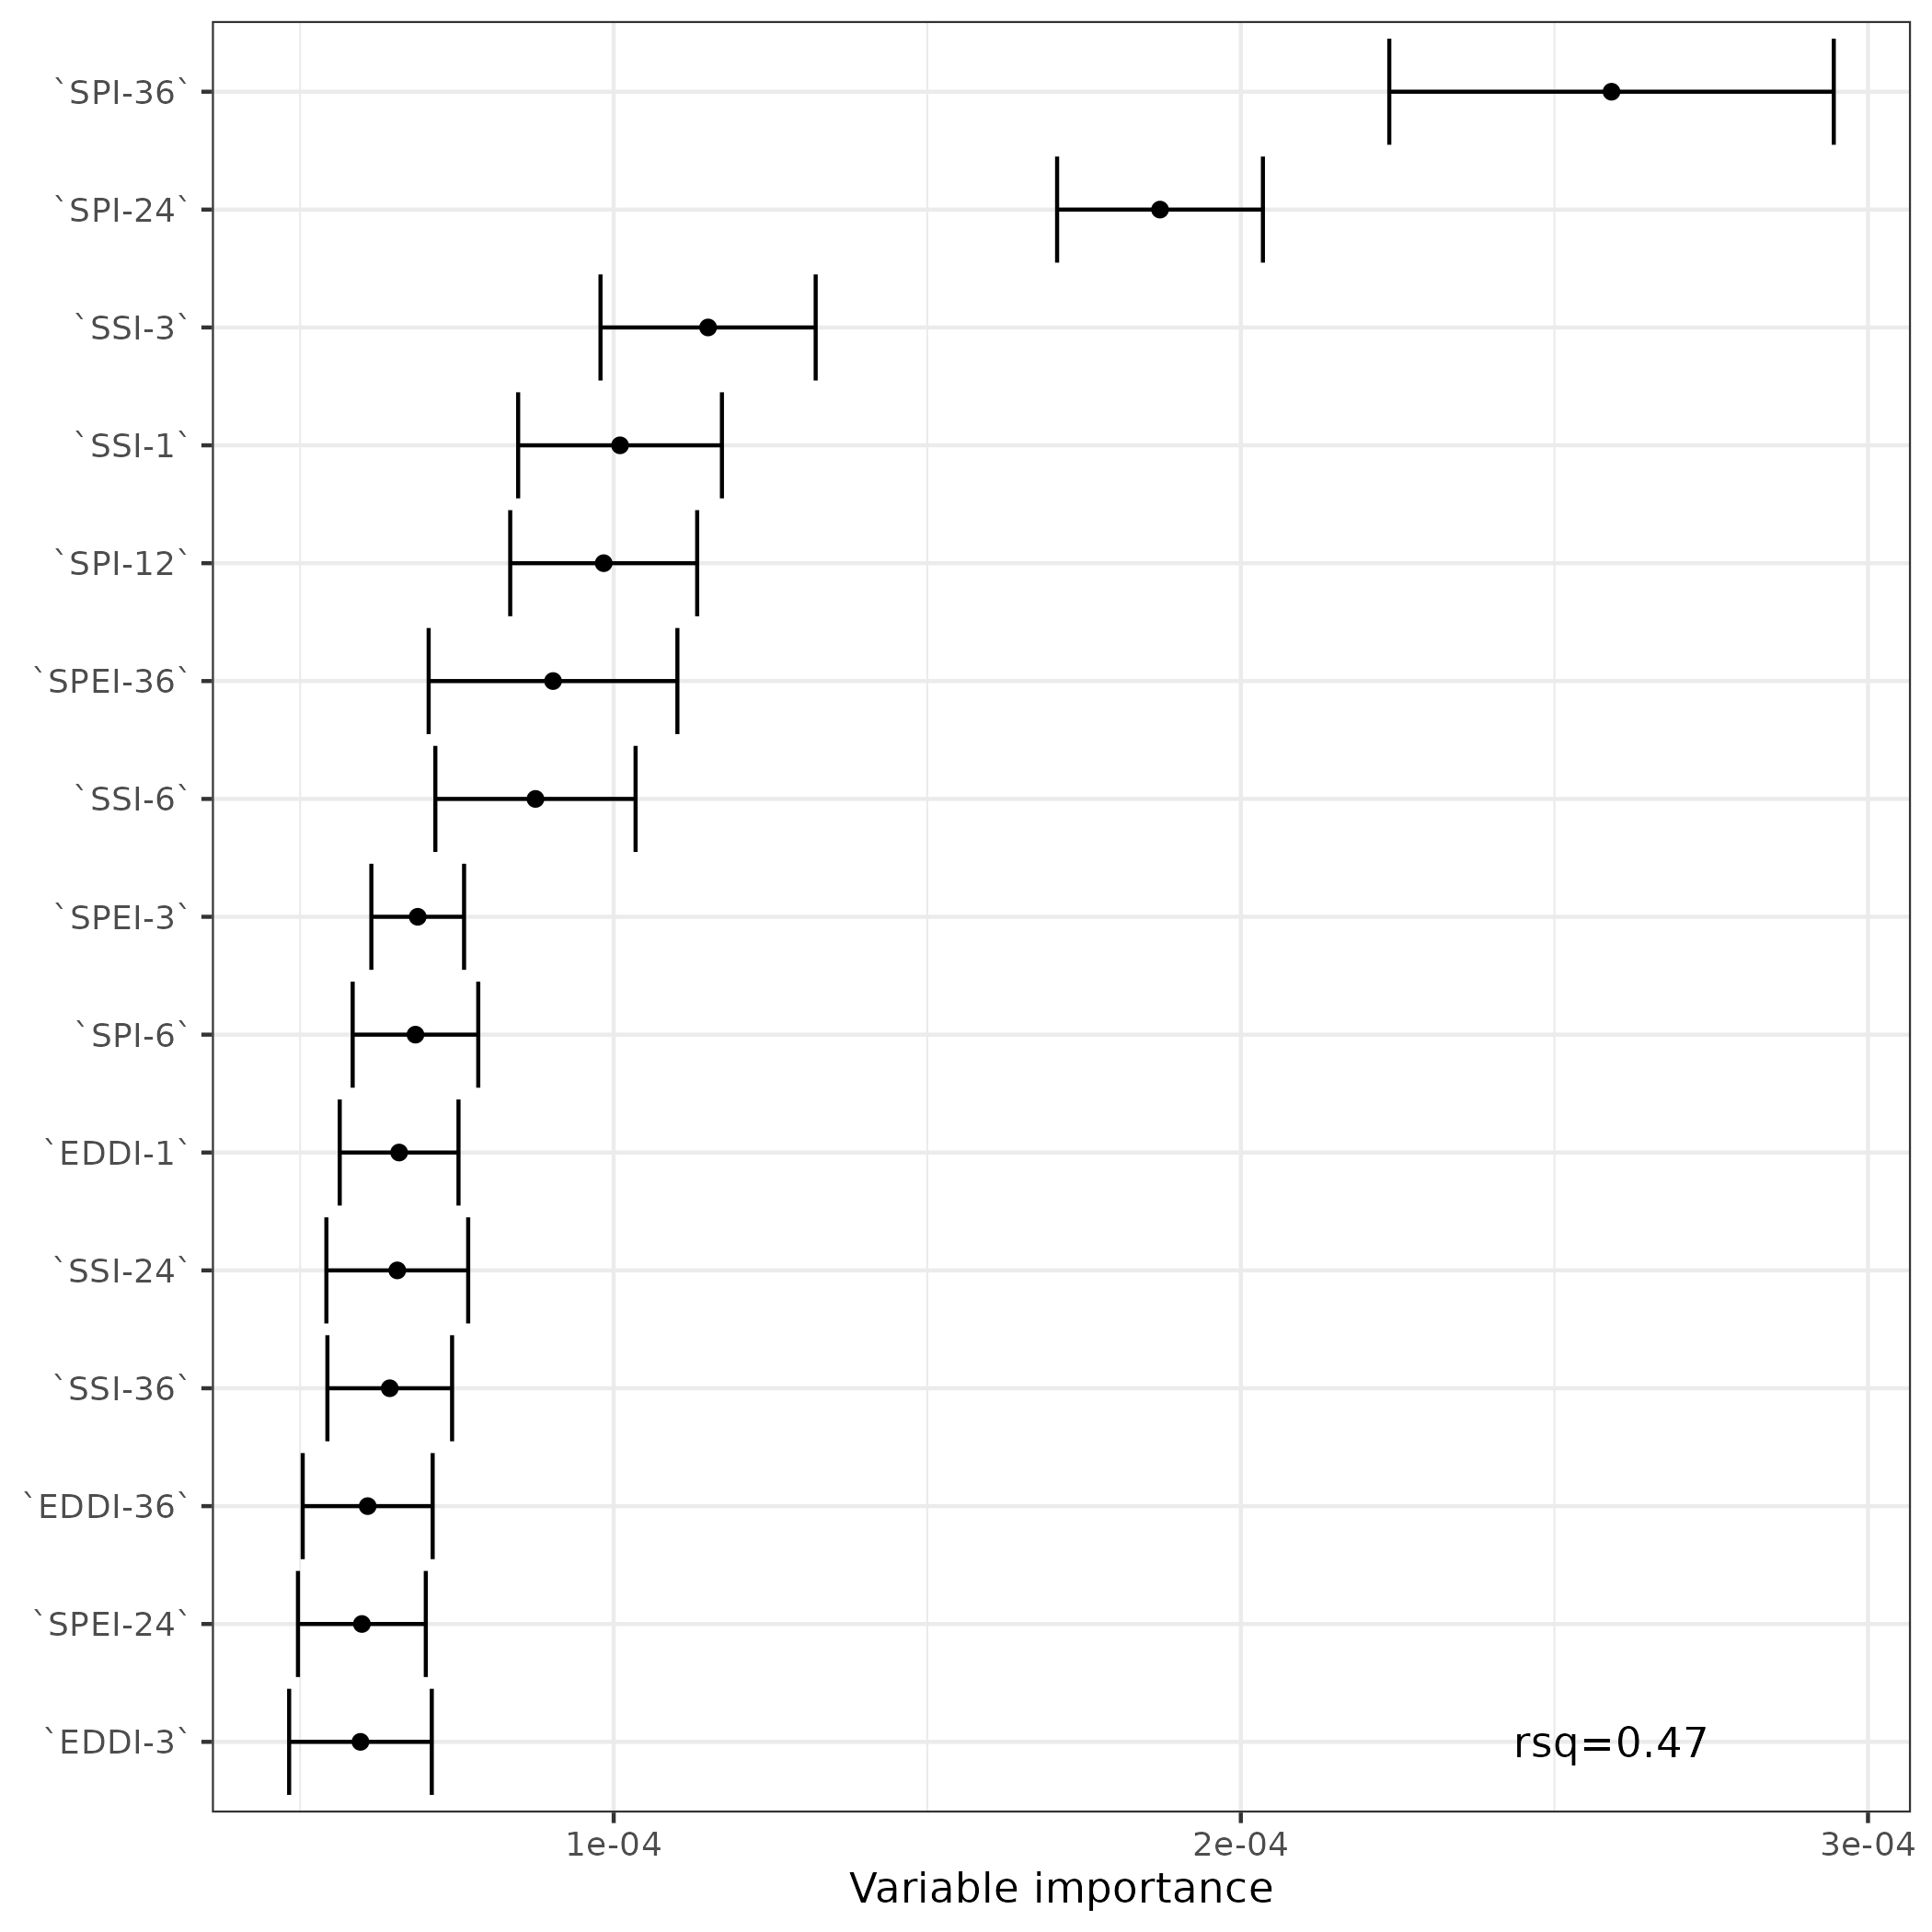
\includegraphics[width=1\textwidth,height=\textheight]{../output/figs/fig_errorbar_resample_random_forest_trends_Shrubland.png}

}

\subcaption{\label{fig-RF_importance-5}Shrubland}

\end{minipage}%
%
\begin{minipage}{0.33\linewidth}

\centering{

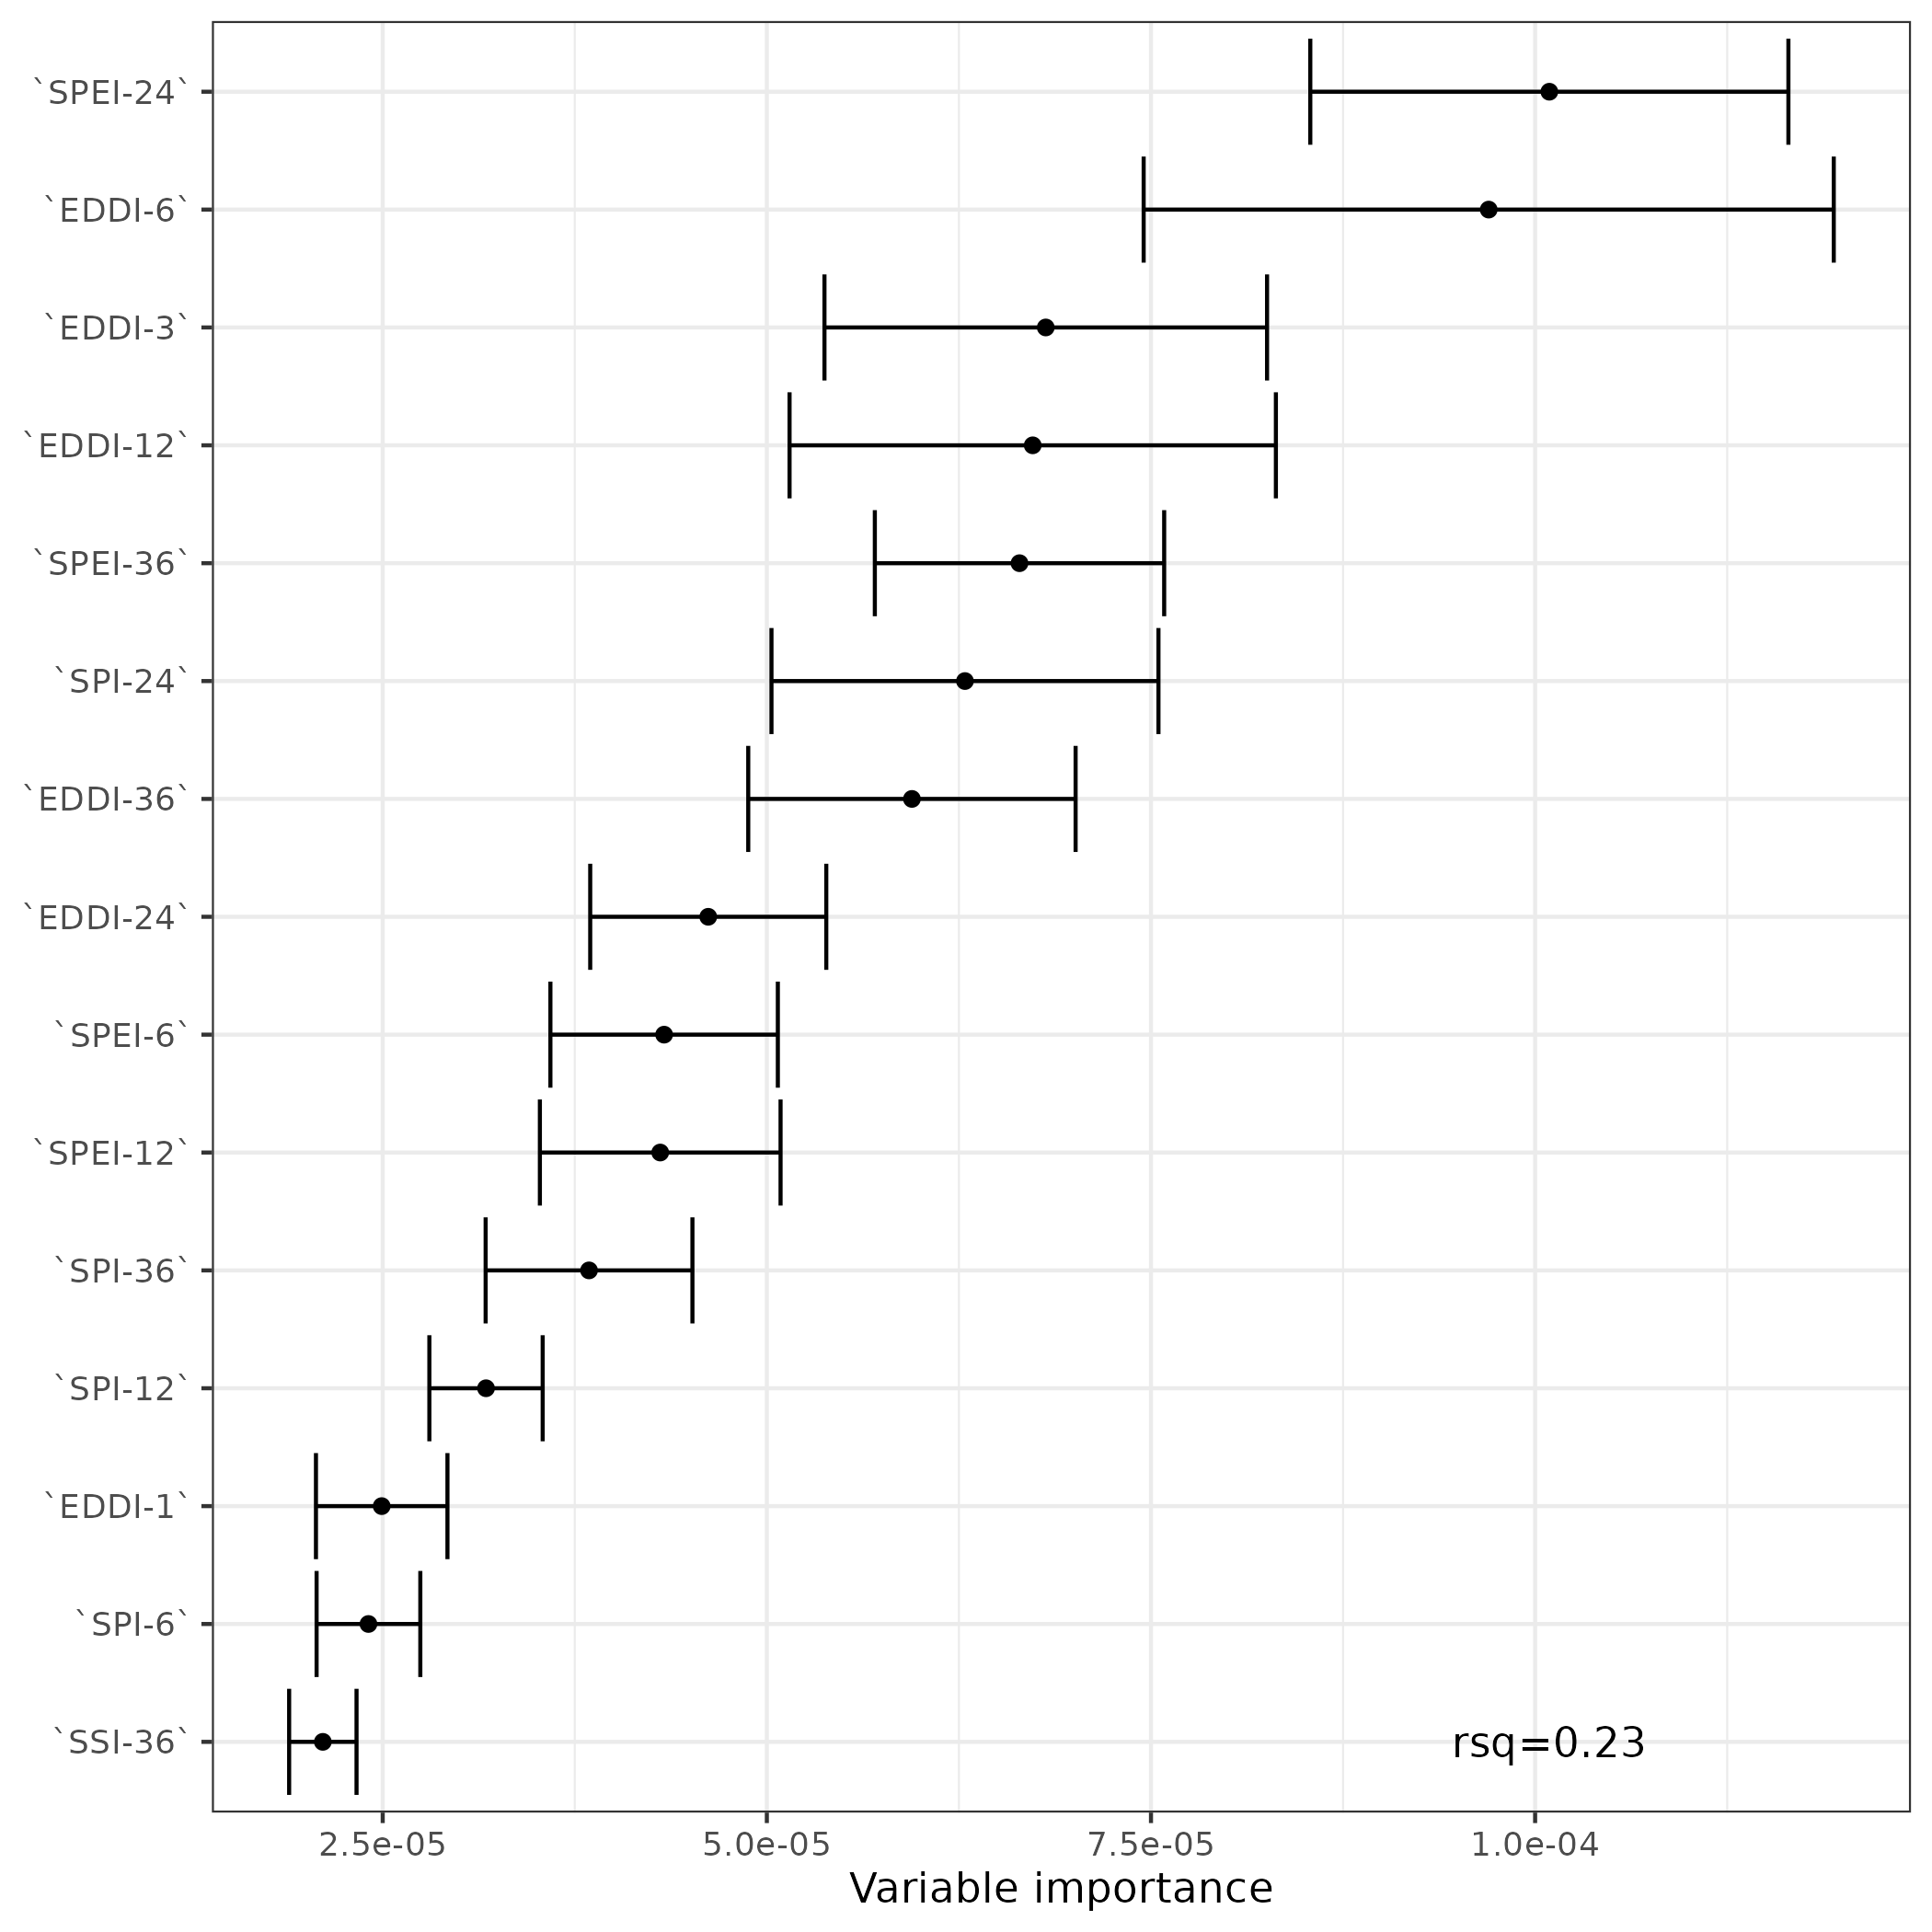
\includegraphics[width=1\textwidth,height=\textheight]{../output/figs/fig_errorbar_resample_random_forest_trends_Barren_land.png}

}

\subcaption{\label{fig-RF_importance-6}Barren Land}

\end{minipage}%

\caption{\label{fig-RF_importance}Error bar for the variables importance
obtained from the 10 resamples folded by the Random Forest used to model
land cover trend using as predictors the trend in drought indices of
water supply, water demand, soil moisture, and vegetation productivity.}

\end{figure*}%

\section{Trend of vegetation
productivity}\label{trend-of-vegetation-productivity}

Figure~\ref{fig-hetmaptrendzcNDVI} shows the average trend for zcNDVI
for 2000-2023 per macrozone and landcover macroclass.

\begin{figure}[!ht]

\centering{

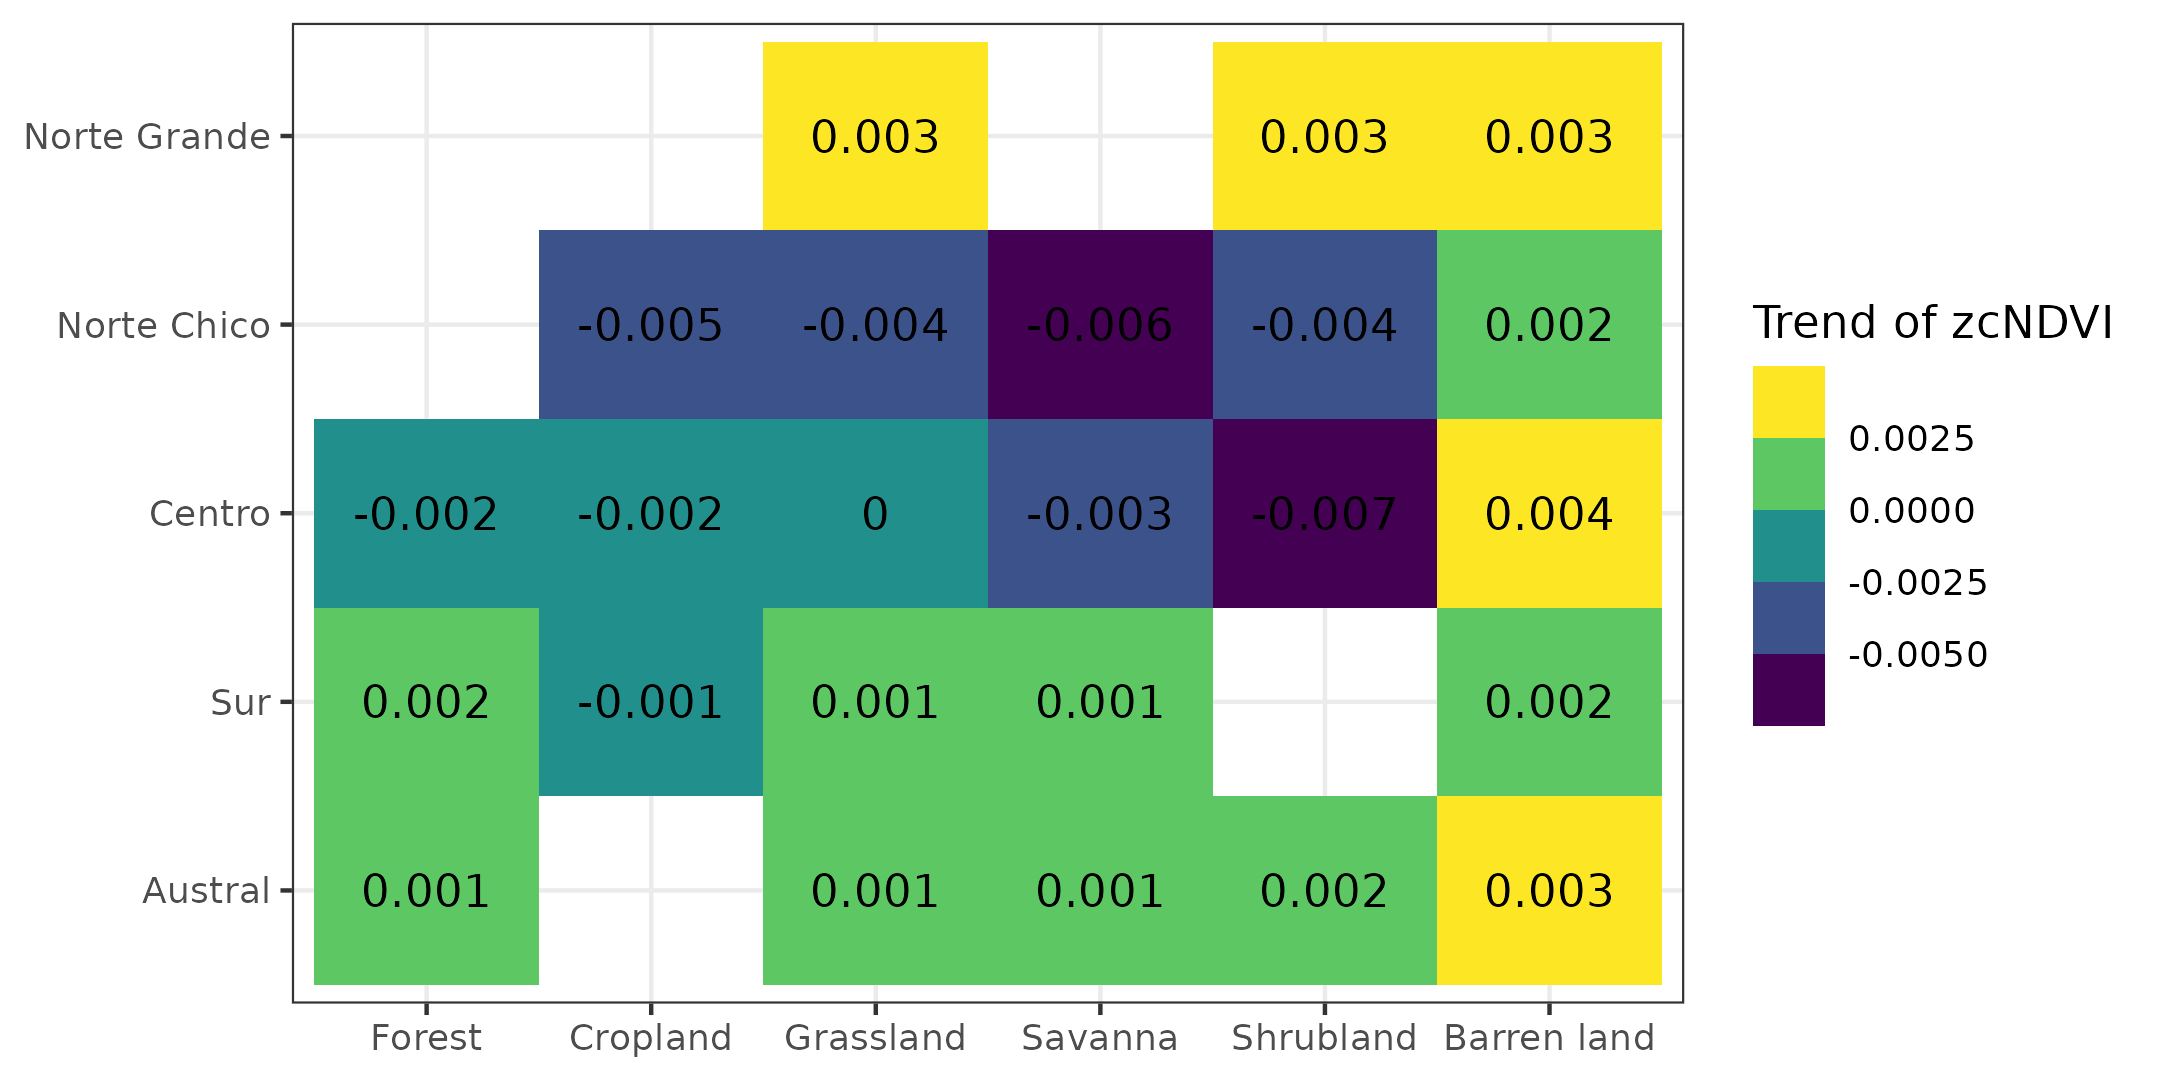
\includegraphics[width=0.75\textwidth,height=\textheight]{../output/figs/heatmap_trends_zcNDVI_macro_landcover.png}

}

\caption{\label{fig-hetmaptrendzcNDVI}Heatmap of trends in zcNDVI for
2000 to 2023 per macrozone and landcover macroclass.}

\end{figure}%

\section{Vegetation productivity}\label{vegetation-productivity}

We analyzed the correlation of zcNDVI for time scales of 1, 3, 6, and 12
months versus net primary production (NPP). We obtained both the zcNDVI
from MOD13A3.061 and the NPP from MOD17A3HGF.061, using MODIS products.
We used the zcNDVI in December to correlate with the annual NPP.
Figure~\ref{fig-r2_npp_zcNDVI} shows a map of the r-squared correlation
between zcNDVI and NPP, and Figure~\ref{fig-hetmap_npp_zcndvi} shows the
aggregated values per macrozone.

\begin{figure}[!ht]

\centering{

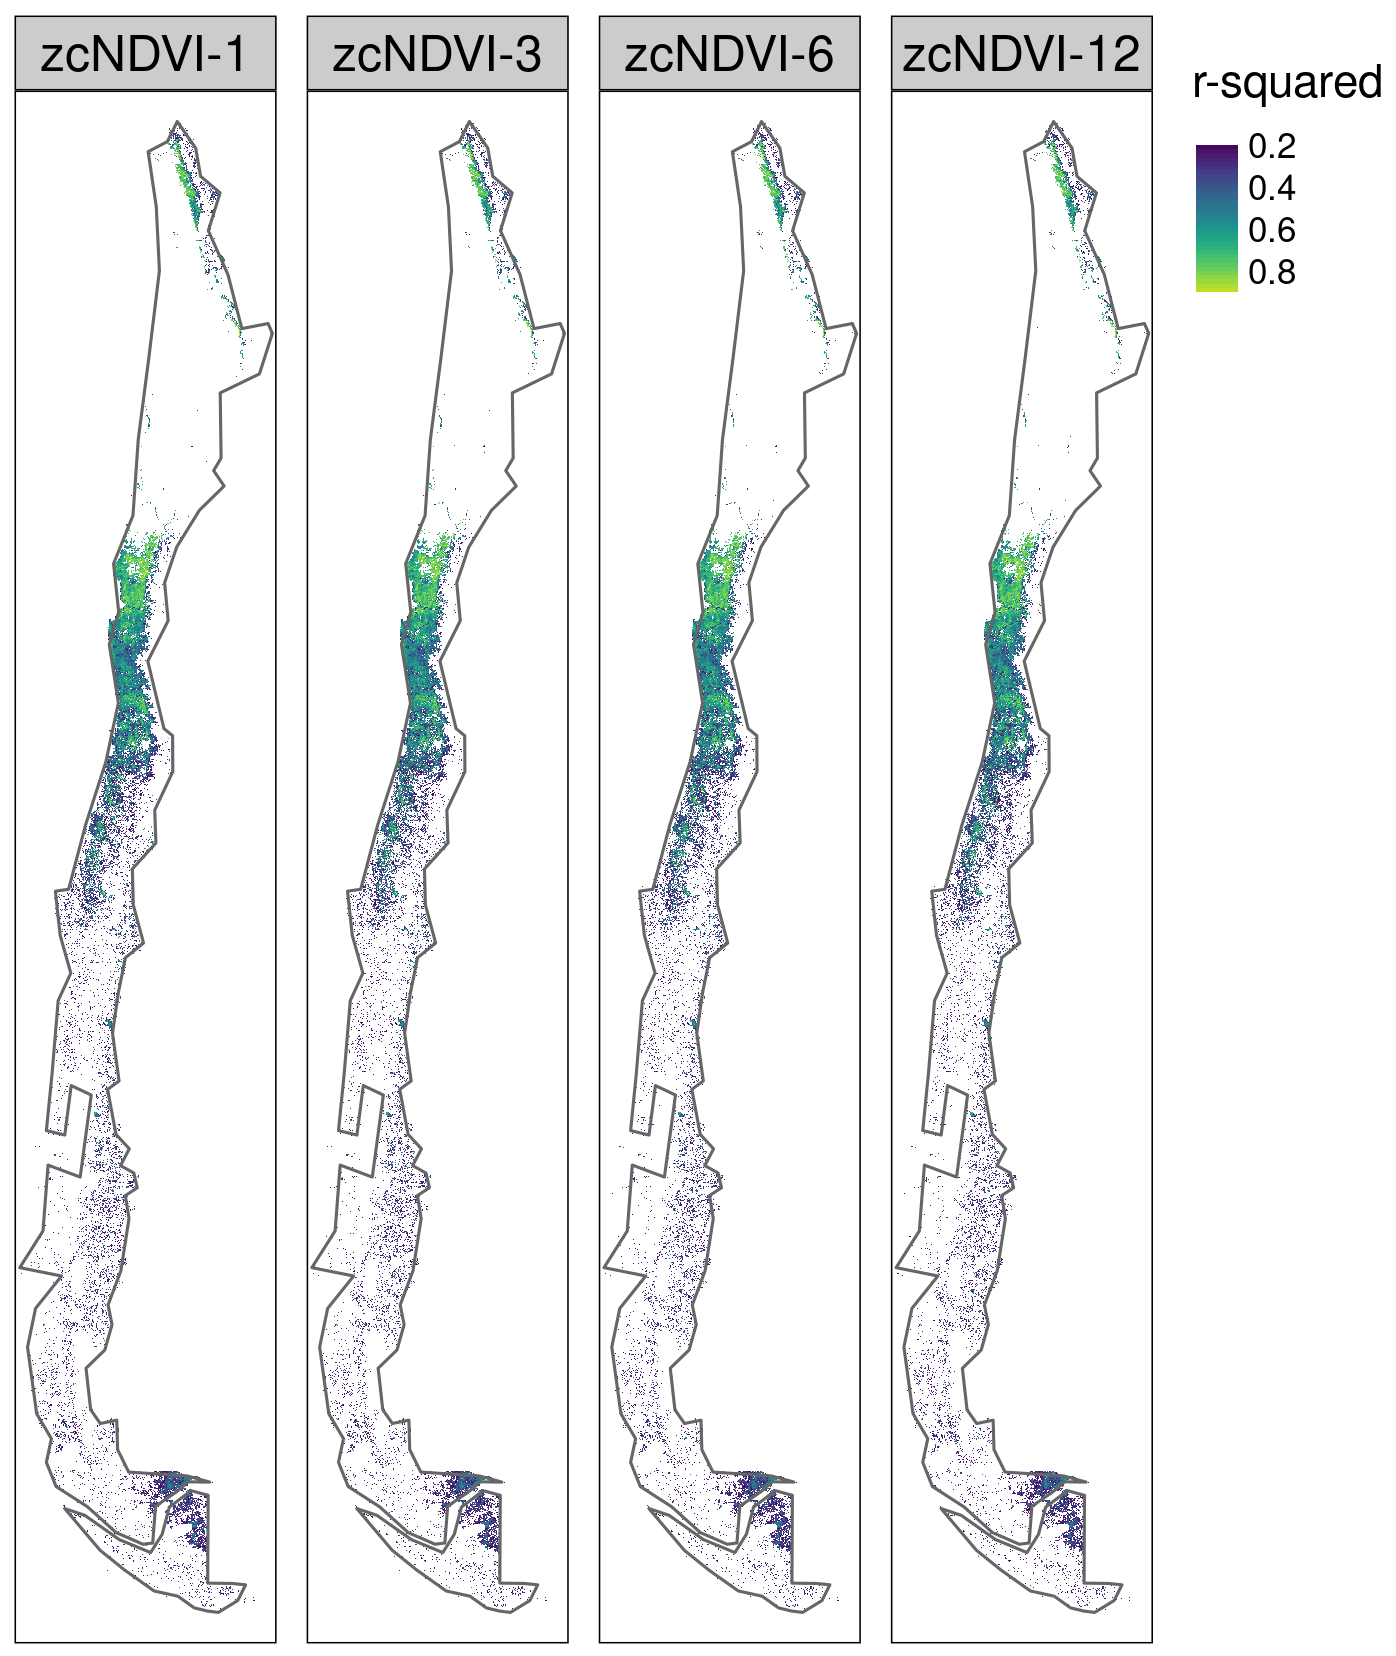
\includegraphics[width=0.75\textwidth,height=\textheight]{../output/figs/map_r2_NPP_vs_zcNDVI.png}

}

\caption{\label{fig-r2_npp_zcNDVI}Spatial variation of the r-squared
values obtained from the yearly correlation of zcNDVI of 1, 3, 6, and 12
months with the net primary productivity (NPP) for continental Chile.}

\end{figure}%

\begin{figure}[!ht]

\centering{

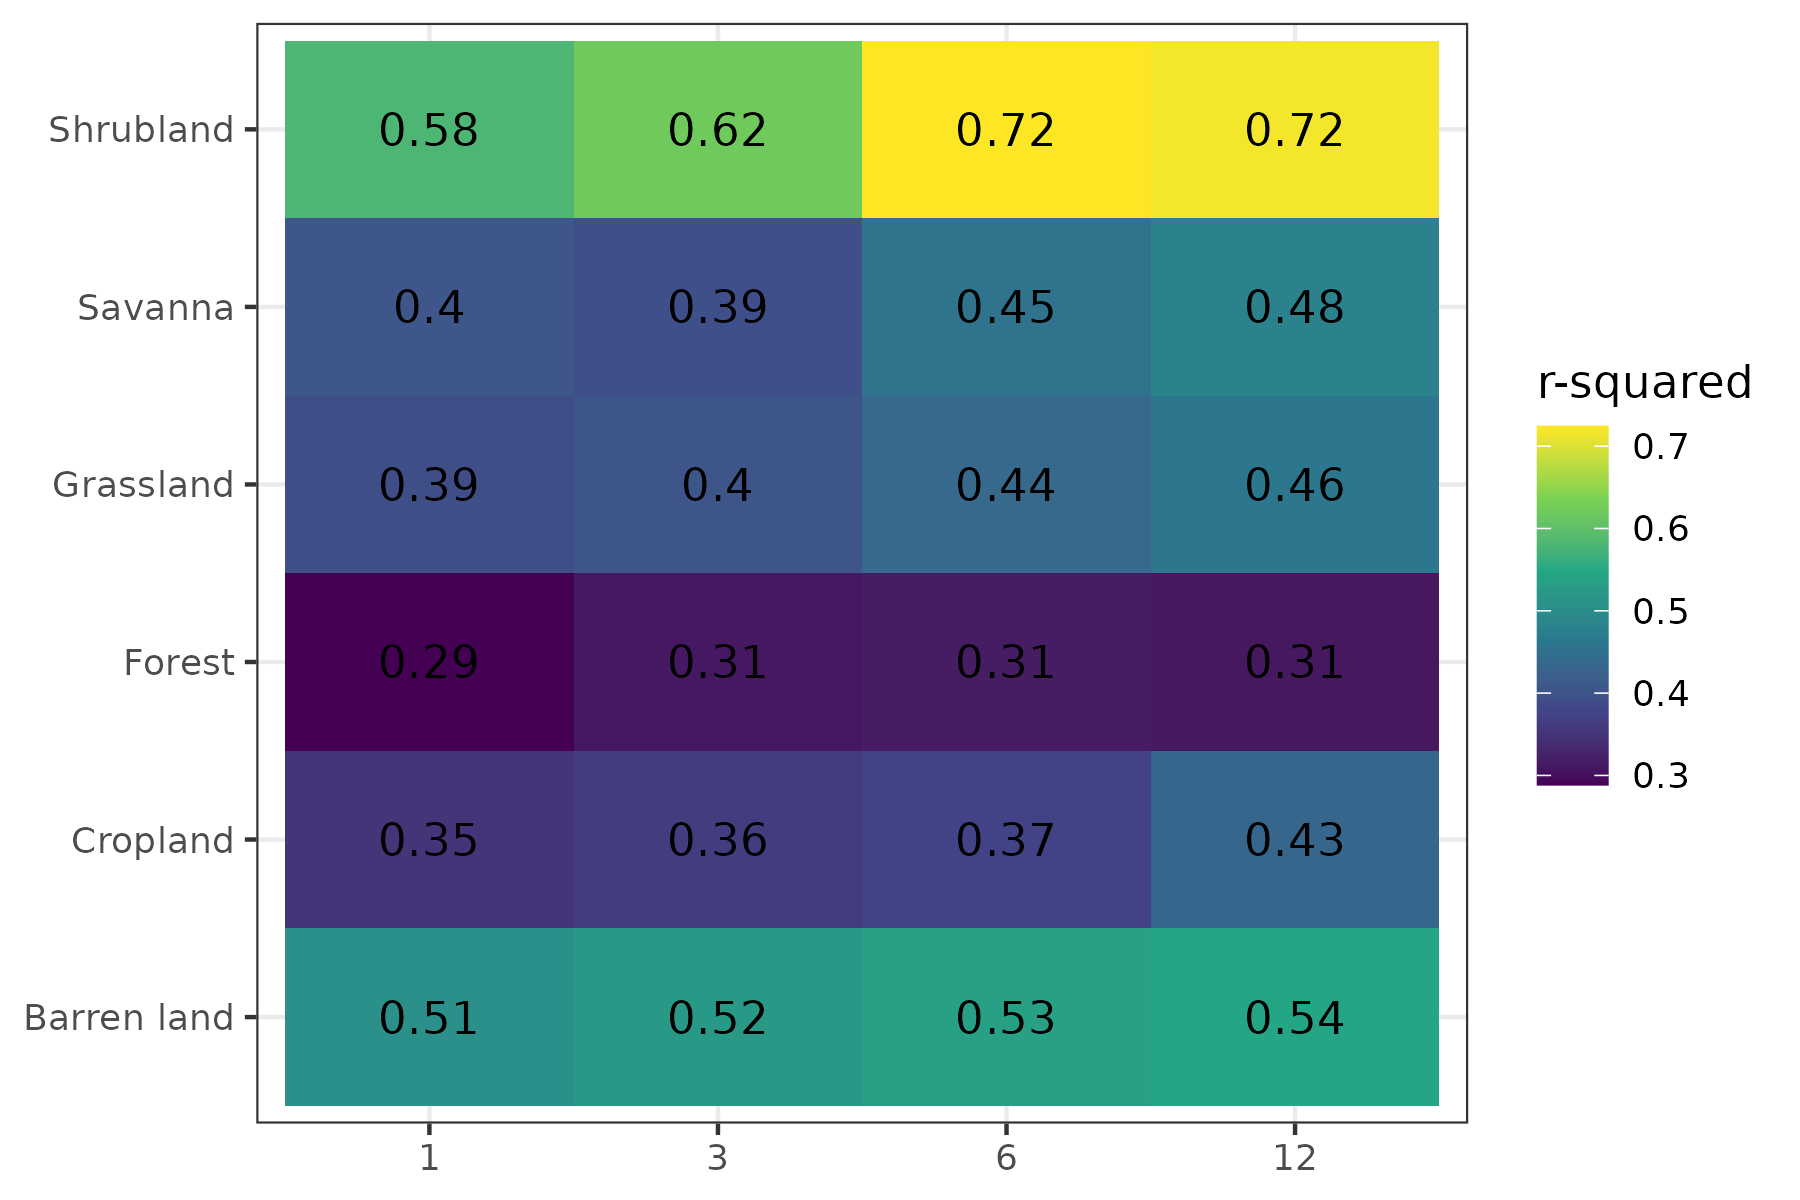
\includegraphics[width=0.5\textwidth,height=\textheight]{../output/figs/heatmap_r2_npp_vs_zcndvi_per_landcover.png}

}

\caption{\label{fig-hetmap_npp_zcndvi}A heatmap showing the r-squared
values obtained from the yearly correlation of zcNDVI of 1, 3, 6, and 12
months with the net primary productivity (NPP) for continental Chile.}

\end{figure}%

\section{Relationship of drought indices and vegetation
productivity}\label{relationship-of-drought-indices-and-vegetation-productivity}

\begin{figure}[H]

{\centering 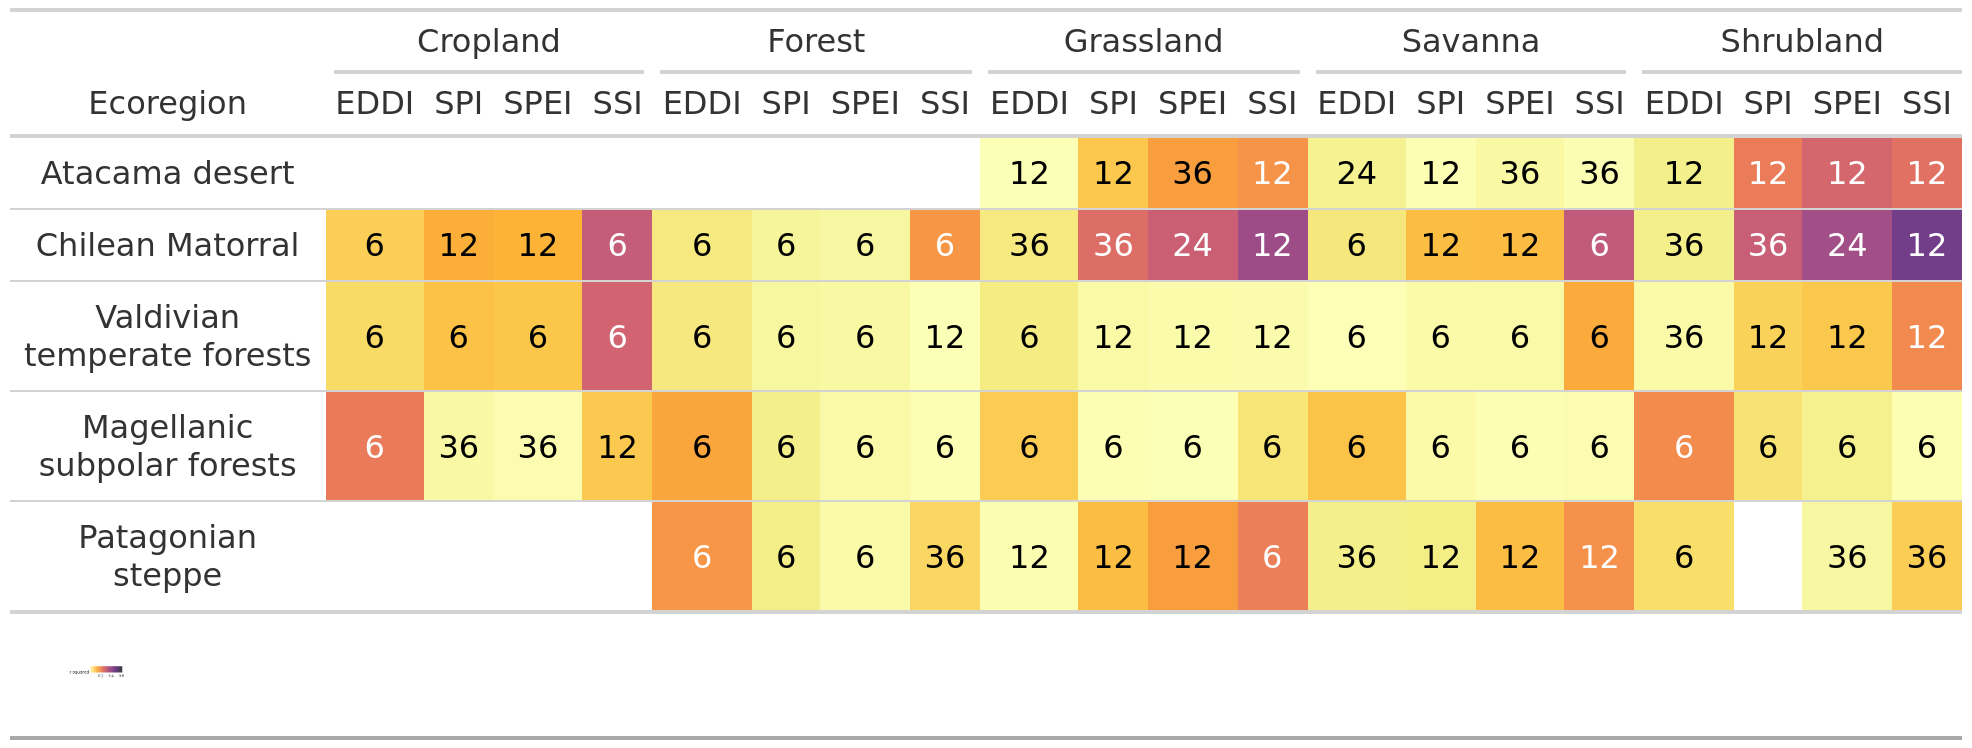
\includegraphics[width=1\textwidth,height=\textheight]{../output/figs/tabla_r_cor_macro_indice.png}

}

\caption{Summary per land cover and study region regarding the
correlation between zcNDVI with the drought indices EDDI, SPI, SPEI, and
SSI for time scales of 1, 3, 6, 12, 24, and 36. The numbers in each cell
indicate the time scale that reached the maximum correlation for the
land cover and macrozone, and the color indicates the strength of the
r-squared obtained with the index and the time scale. Cells without
values indicate that the land cover type was not significant in that
macrozone.}

\end{figure}%

\newpage

\section*{References}\label{references}
\addcontentsline{toc}{section}{References}

\renewcommand{\bibsection}{}
\bibliography{references.bib}




\end{document}
